\documentclass[tikz,border=6pt]{standalone}
\usepackage{amsmath,amssymb,mathtools,physics,bm,nicefrac,wasysym}
\usepackage{xcolor}

\definecolor{colone}{RGB}{180,60,60}
\definecolor{coltwo}{RGB}{60,110,180}
\definecolor{colthree}{RGB}{60,140,80}

\definecolor{accent}{HTML}{A13D2C}
\definecolor{accent2}{HTML}{2B5F6B}
\definecolor{muted}{HTML}{5A564F}
\definecolor{panel}{HTML}{F8F6F0}
\definecolor{linecol}{HTML}{D8D2C4}
\definecolor{ink}{HTML}{1E1C1A}
\definecolor{astroblue}{HTML}{1B4F72}
\definecolor{astrodark}{HTML}{17202A}
\definecolor{sunyellow}{HTML}{E8A33D}

\usetikzlibrary{calc,arrows.meta,positioning,decorations.pathreplacing,decorations.markings,angles,quotes,shapes.geometric}
\usepackage{tikz-3dplot}

\newcommand{\vecr}{\vec r}
\newcommand{\vecL}{\vec L}
\newcommand{\vecA}{\vec A}
\newcommand{\vecf}{\vec f}
\newcommand{\vecF}{\vec F}
\newcommand{\vecp}{\vec p}
\newcommand{\avg}[1]{\left\langle #1\right\rangle}
\newcommand{\vecx}{\vec x}
\newcommand{\hatn}{\hat n}
\newcommand{\rhat}{\hat r}
\newcommand{\phihat}{\hat\phi}
\newcommand{\thetahat}{\hat\theta}
\newcommand{\note}[1]{\textcolor{blue!60!black}{\textit{[#1]}}}

\newcommand{\LST}{\mathrm{LST}}
\newcommand{\GST}{\mathrm{GST}}
\newcommand{\GMST}{\mathrm{GMST}}
\newcommand{\GAST}{\mathrm{GAST}}
\newcommand{\LMST}{\mathrm{LMST}}
\newcommand{\LAST}{\mathrm{LAST}}
\newcommand{\UT}{\mathrm{UT}}
\newcommand{\UTC}{\mathrm{UTC}}
\newcommand{\TAI}{\mathrm{TAI}}
\newcommand{\TT}{\mathrm{TT}}
\newcommand{\TDB}{\mathrm{TDB}}
\newcommand{\JD}{\mathrm{JD}}
\newcommand{\MJD}{\mathrm{MJD}}
\newcommand{\EoT}{\mathrm{EoT}}
\newcommand{\SNR}{\mathrm{SNR}}
\newcommand{\RON}{\mathrm{RON}}



\begin{document}
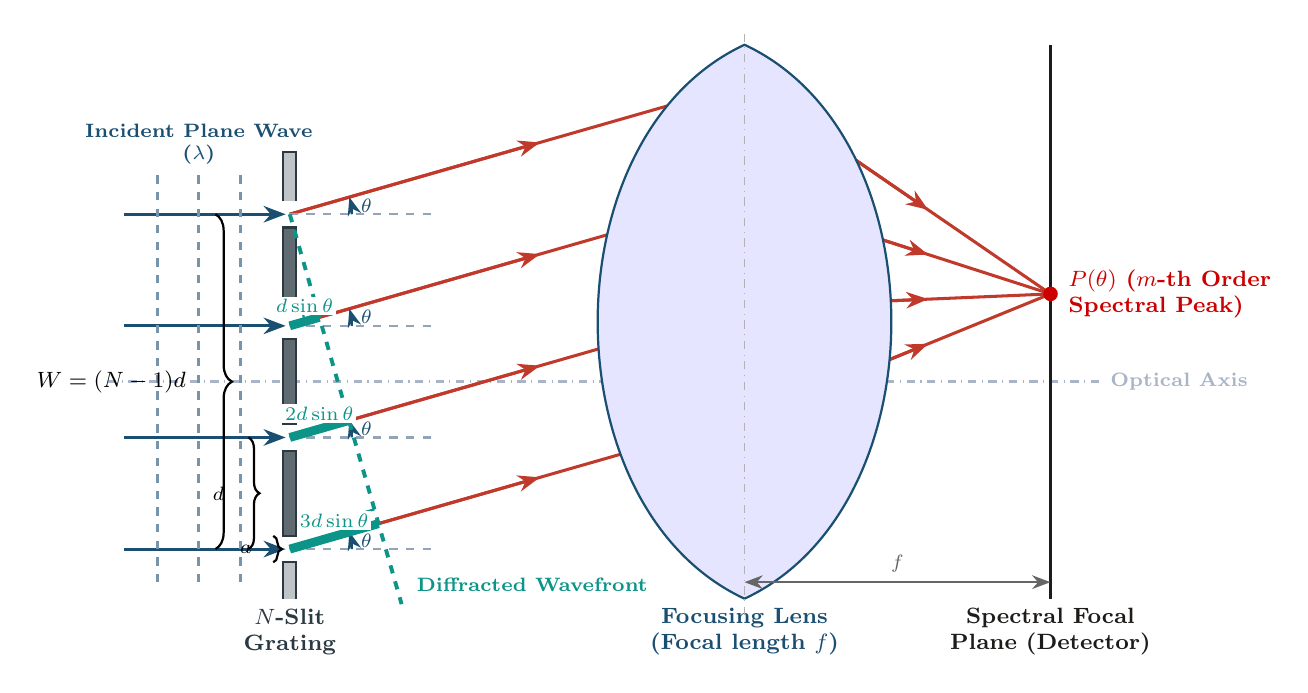
\begin{tikzpicture}[scale=1.05, >=Stealth]
    % Parameters
    \def\Nslits{4}
    \def\d{1.35}     % Slit pitch
    \def\a{0.32}     % Slit width
    \def\thetaDeg{16} % Diffraction angle (clean, modest angle)
    \def\lensX{5.5}  % Distance to lens
    \def\screenX{9.2} % Distance to screen
    \def\yMid{2.025} % (0 + 3*1.35)/2 = 2.025 (center of grating & optical axis)
    
    \pgfmathsetmacro{\fLen}{\screenX - \lensX}
    \pgfmathsetmacro{\focalY}{\yMid + \fLen*tan(\thetaDeg)}
    
    % Colors
    \definecolor{gratingCol}{HTML}{2B3A42}
    \definecolor{rayCol}{HTML}{C0392B}
    \definecolor{waveCol}{HTML}{0D9488}
    \definecolor{guideCol}{HTML}{94A3B8}
    \definecolor{accentCol}{HTML}{1B4F72}
    
    % Optical Axis
    \draw[dashdotted, guideCol!80, line width=0.9pt] (-2.2, \yMid) -- (\screenX+0.6, \yMid) 
        node[right, font=\scriptsize\bfseries\color{guideCol!90!black}] {Optical Axis};

    % Grating Plane at x = 0
    \fill[gratingCol!30] (-0.08, -0.6) rectangle (0.08, {-0.5*\a});
    \draw[thick, gratingCol] (-0.08, -0.6) -- (-0.08, {-0.5*\a}) -- (0.08, {-0.5*\a}) -- (0.08, -0.6);
    
    \fill[gratingCol!30] (-0.08, {3*\d + 0.5*\a}) rectangle (0.08, 4.8);
    \draw[thick, gratingCol] (-0.08, {3*\d + 0.5*\a}) -- (-0.08, 4.8) -- (0.08, 4.8) -- (0.08, {3*\d + 0.5*\a});
    
    % Slits and rays
    \foreach \i in {0, 1, 2, 3} {
        \pgfmathsetmacro{\yCenter}{\i*\d}
        \coordinate (S\i) at (0, \yCenter);
        
        \draw[->, line width=1.1pt, astroblue] (-2.0, \yCenter) -- (-0.05, \yCenter);
        
        \pgfmathsetmacro{\yLens}{\yCenter + \lensX*tan(\thetaDeg)}
        \coordinate (L\i) at (\lensX, \yLens);
        \draw[line width=1.1pt, rayCol] (S\i) -- (L\i);
        \draw[->, line width=1.1pt, rayCol] (S\i) -- ($(S\i)!0.55!(L\i)$);
        
        \coordinate (P) at (\screenX, \focalY);
        \draw[line width=1.1pt, rayCol] (L\i) -- (P);
        \draw[->, line width=1.1pt, rayCol] (L\i) -- ($(L\i)!0.6!(P)$);
        
        \ifnum\i<3
            \pgfmathsetmacro{\yTop}{\yCenter + 0.5*\a}
            \pgfmathsetmacro{\yNextBottom}{(\i+1)*\d - 0.5*\a}
            \fill[gratingCol!75] (-0.08, \yTop) rectangle (0.08, \yNextBottom);
            \draw[thick, gratingCol] (-0.08, \yTop) rectangle (0.08, \yNextBottom);
        \fi
    }
    
    % Incoming wavefronts
    \foreach \xw in {-1.6, -1.1, -0.6} {
        \draw[line width=1.0pt, astroblue!60, dashed] (\xw, -0.4) -- (\xw, 4.6);
    }
    \node[astroblue, font=\bfseries\scriptsize, align=center] at (-1.1, 4.9) {Incident Plane Wave\\($\lambda$)};

    % Normal reference lines & angle arcs at each slit
    \foreach \i in {0, 1, 2, 3} {
        \draw[dashed, guideCol, thick] (S\i) -- ++(1.8, 0);
        \draw[->, thick, accentCol] ({0.75}, {\i*\d}) arc (0:\thetaDeg:0.75);
        \node[accentCol, font=\scriptsize\bfseries, right] at ({0.75*cos(0.5*\thetaDeg)}, {\i*\d + 0.75*sin(0.5*\thetaDeg)}) {$\theta$};
    }
    
    % Diffracted Wavefront
    \foreach \i in {0, 1, 2} {
        \pgfmathsetmacro{\ti}{(3 - \i)*\d*sin(\thetaDeg)}
        \pgfmathsetmacro{\wXi}{\ti*cos(\thetaDeg)}
        \pgfmathsetmacro{\wYi}{\i*\d + \ti*sin(\thetaDeg)}
        \coordinate (W\i) at ({\wXi}, {\wYi});
        \draw[line width=3.2pt, waveCol] (S\i) -- (W\i);
        
        \pgfmathsetmacro{\sqSize}{0.18}
        \draw[thick, waveCol] 
            ($(W\i) + ({-\sqSize*cos(\thetaDeg)}, {-\sqSize*sin(\thetaDeg)})$) -- 
            ++({-\sqSize*sin(\thetaDeg)}, {\sqSize*cos(\thetaDeg)}) -- 
            ($(W\i) + ({-\sqSize*sin(\thetaDeg)}, {\sqSize*cos(\thetaDeg)})$);
    }
    
    \coordinate (Wext) at ($(S3)!1.26!(W0)$);
    \draw[dashed, line width=1.4pt, waveCol] (S3) -- (Wext);
    \node[waveCol, font=\bfseries\scriptsize, above right=1pt and 2pt] at (Wext) {Diffracted Wavefront};
        
    \node[waveCol, font=\bfseries\scriptsize, above=2pt, fill=white, inner sep=1pt] at ($(S0)!0.5!(W0)$) {$3d\sin\theta$};
    \node[waveCol, font=\bfseries\scriptsize, above=2pt, fill=white, inner sep=1pt] at ($(S1)!0.5!(W1)$) {$2d\sin\theta$};
    \node[waveCol, font=\bfseries\scriptsize, above=2pt, fill=white, inner sep=1pt] at ($(S2)!0.5!(W2)$) {$d\sin\theta$};

    % Focusing Lens
    \draw[thick, fill=blue!10, draw=astroblue] 
        (\lensX, -0.6) to[out=25, in=-25] (\lensX, 6.1) 
        to[out=-155, in=155] (\lensX, -0.6);
    \node[astroblue, font=\bfseries\footnotesize, align=center] at (\lensX, -1.0) {Focusing Lens\\(Focal length $f$)};
    \draw[dashdotted, gray!60] (\lensX, -0.8) -- (\lensX, 6.3);

    % Spectral Focal Plane Screen
    \draw[very thick, ink] (\screenX, -0.6) -- (\screenX, 6.1);
    \node[ink, font=\bfseries\footnotesize, align=center] at (\screenX, -1.0) {Spectral Focal\\Plane (Detector)};
    
    \fill[red!80!black] (P) circle (2.5pt);
    \node[right=3pt, red!80!black, font=\bfseries\footnotesize, align=left] at (P) {$P(\theta)$ ($m$-th Order\\Spectral Peak)};

    \draw[<->, thick, gray!80!black] (\lensX, -0.4) -- (\screenX, -0.4) 
        node[midway, above, font=\scriptsize\bfseries] {$f$};

    \draw[decorate, decoration={brace, amplitude=3pt, mirror}, thick]
        (-0.2, -0.16) -- (-0.2, 0.16) node[midway, left=4pt, font=\scriptsize\bfseries] {$a$};
        
    \draw[decorate, decoration={brace, amplitude=4pt, mirror}, thick]
        (-0.5, 0) -- (-0.5, \d) node[midway, left=5pt, font=\scriptsize\bfseries] {$d$};

    \draw[decorate, decoration={brace, amplitude=6pt, mirror}, thick]
        (-0.9, 0) -- (-0.9, {3*\d}) node[midway, left=7pt, font=\footnotesize\bfseries] {$W = (N-1)d$};

    \node[gratingCol, font=\bfseries\footnotesize, align=center] at (0, -1.0) {$N$-Slit\\Grating};
\end{tikzpicture}
\end{document}
